% --
% my dataset

\subsection{My own Dataset}\label{sec:exp_dataset_my}
This dataset is created by the author of this thesis and contain 5 speech command samples from the words (classes) \enquote{left}, \enquote{right}, \enquote{up}, \enquote{down} and \enquote{go}.
Its purpose is mainly as test set in evaluating trained models.
It is important to mention that none of the self recorded files are used within the training set, so that it the neural networks performance on unseen data is evaluated.
All examples of my own dataset are illustrated in \rfig{exp_dataset_wav_grid_my} in raw audio format.
\begin{figure}[!ht]
  \centering
    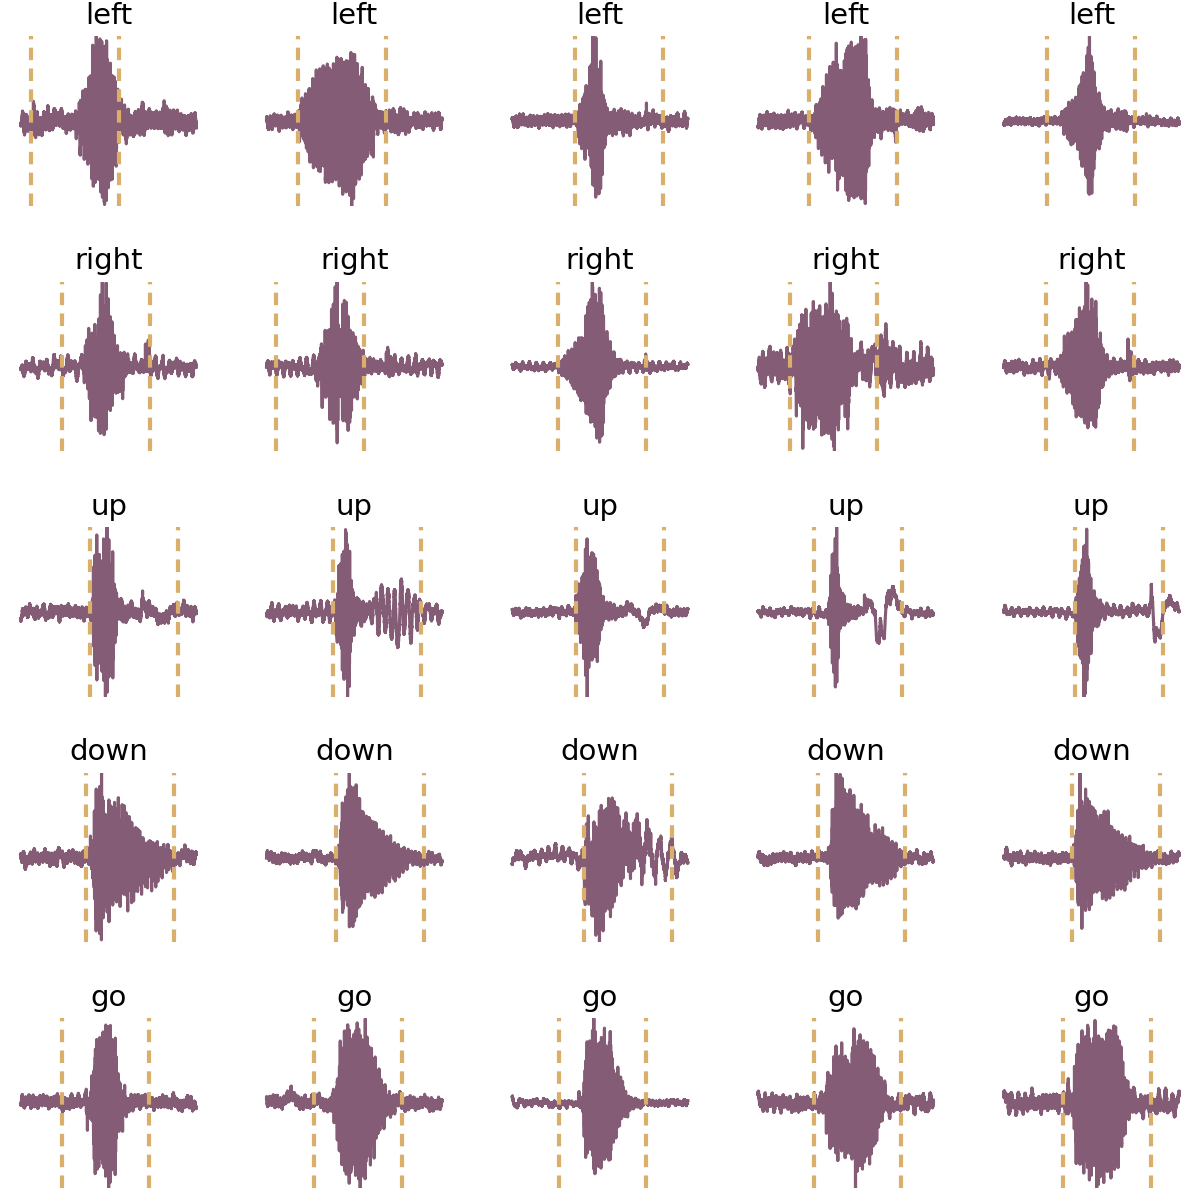
\includegraphics[width=0.65\textwidth]{./5_exp/figs/exp_dataset_wav_grid_my}
  \caption{Self recorded files of the \equote{my dataset} in raw audio format.}
  \label{fig:exp_dataset_wav_grid_my}
\end{figure}
\FloatBarrier
\noindent
The examples per class are spoken with different emphasis and stress on individual phonemes, such that they do not sound the same.
Also the prolongation of the words are different, such that in one example the word is fast and in the other its slow spoken.
The emphasis and prolongation ensure the diversity of the dataset and it turned out that it is not easy for neural networks to gain a $100\%$ classification rate upon it, even though there is only one and the same speaker.
